\subsection{Smart Locks}
\label{sec:sota_smart_locks}

	relevant: \cite{Ye2017}\cite{Fuller2017}\cite{Rose2016}\cite{Ho2016}
	\missingfigure{Bilder von Smart Lock-Systemen}
	
	\begin{itemize}
	    \item keine Smart Locks, die einfach ein Türschloss mit einem Ziffernblock ersetzen oder nicht mit anderen Geräten in irgendeiner Weise verbinden, da sie sich fundamental von herkömmlichen \gls{iot}-Geräten unterscheiden\cite{Ho2016}
	    \item keine Smart Locks, die sich nicht direkt oder über ein Gateway mit dem Internet verbinden können\cite{Ho2016}
	\end{itemize}
	
	\subsubsection{Typische Architekturen und Gemeinsamkeiten}
	    Nach \citeauthor{Ye2017}:
		\begin{itemize}
			\item Türschloss, häufig elektromagnetisch. Das Öffnen erfolgt primär elektronisch. Alternativ lässt sich das Schluss entweder mit einem Keyfob (einem Schlüsselanhänger, auf dem sich ein digitaler Schlüssel befindet) oder einem physischen Schüssel öffnen.
			\item Mobile Applikation auf einem Smartphone
			\item Herstellereigener Remote Server, auf dem sich in den meisten Fällen eine authoritative Liste aller Nutzer, sowie deren Rechte befindet
		\end{itemize}

		Bestandteile nach \citeauthor{Ho2016}:
		\begin{itemize}
		    \item elektronisch erweitertes Schloss, welches an der Außenseite einer Tür\todo[color=orange]{besser formulieren} angebracht ist
		    \item als Rückfalllösung ist bei allen ein Smart Locks traditionelles Schlüsselloch, welches sich mit einem physischen Schlüssel öffnen lässt.
		    \item das Schloss lässt sich von innen manuell bedient werden
		    \item mobiles Gerät mit entsprechender App, über welche das Schloss elektronisch kontrolliert werden kann, sowie Administration möglich ist
		    \item Remote Webserver des Herstellers
		    \item Weboberfläche zur Administration
		\end{itemize}

		Funktion nach \citeauthor{Ho2016}
		\begin{itemize}
		    \item Um das Schloss zu kontrollieren installiert der Nutzer eine App, häufig herstellerspezifisch, je nach Schloss auf ihrem Mobilgerät.
		    \item Der Nutzer erstellt ein Nutzerkonto auf dem Server des Herstellers
		    \item Nutzer pairt sein Geräte mit dem Schloss mittels eines lokalen kabellosen Kanals, wie \gls{ble}
		    \item Die Identifikation der verschiedenen Nutzer erfolgt entweder mittels E-Mailadresse oder Telefonnummer.
		    \item Die Smart Locks enthalten eine eingebaute Funktion, um jegliche Zugriffe zu protokollieren.
		    \item Lediglich der Nutzer mit der Rolle des Owners kann diese Protokolle einsehen.
		    \item Das elektronische Öffnen und Schließen erfolgt mittels eines Buttons in der App.
		        Funktion, um das Schloss ohne Interaktion des Nutzers zu öffnen.
		        Entweder komplett automatisch bei Annäherung oder nach berühren einer Schaltfläche auf dem Schloss.
		        Dabei wird geprüft, ob der Nutzer authorisiert ist.
		\end{itemize}

        Kommunikation nach \citeauthor{Ho2016}:
        \begin{enumerate}
            \item In \fref{fig:gateway} abgebildet: Smart Lock hat keine Internetverbindung.
                Endgerät des Nutzers übernimmt die Funktion eines Proxy/Gateway, welches Informationen zwischen dem Smart Lock und den Servern des Herstellers überträgt.
                Dies setzt voraus, dass sich das Endgerät in Kommunikationsreichweite für das jeweilige Protokoll (bspw. \gls{ble}) befindet.
            \item Direkte Internetverbindung des Smart Locks zur Kommunikation mit dem Server des Herstellers mittels eingebautem Wifi-Modem, welches sich mit dem Netzwerk des Nutzers verbindet.
                Die Informationen über Rechtevergaben und Gerätezustand etc. werden hier allerdings über das Internet und nicht über lokale Kommunikation (wie \gls{ble}) übertragen.
        \end{enumerate}
        
		\begin{figure}[H]
			\centering
			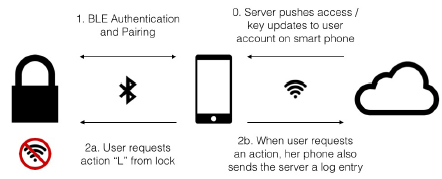
\includegraphics[width=0.5\textwidth]{paperNotes/ho2016_components}
			\caption{Kommunikation zwischen Komponenten des Smart Lock Systems von August}
			\label{fig:gateway}
		\end{figure}

        Rollen und Rechteverteilungen\cite{Ye2017}\cite{Ho2016}:
		\begin{itemize}
			\item Rollen: Owner(Grant, Revoke, Lock/Unlock, Admin Features wie Zugriffshistorie), Resident(Lock/Unlock), wiederkehrender Gast (nur Lock/Unlock zu bestimmten Zeitfenstern), temporärer Gast(Lock/Unlock für eine bestimmte Zeit wie 24 Stunden)
			    Die Rolle des Owners wird jenem Gerät vergeben, das sich nach Installation des Smart Locks als erstes mittels \gls{ble} (oder bei einigen Modellen über W-LAN) verbindet.
			    Die Owner-Rolle kann auf diesem Wege nur einmal vergeben werden.
			    Bei Wechsel des Besitzers muss das Smart Lock zurückgesetzt werden.
			    Rollen wieder zu entfernen und somit anderen Nutzers wieder die Rechte zu entziehen, muss Owner sein.
			    Um die Rechte eines Owners bei einem verlorenen oder gestohlenen zu entziehen, wird entweder eine "Lost Phone"-Funktion angeboten oder ein anderer Nutzer mit der Rolle des Owners entzieht dem nicht mehr vorhandenen Gerät die Rolle.
			\item Permissions: Lock/Unlock, Lock Activity, Guest List, User Invitation (new Users), User Level Control (update User Role), User Permission Control (set time slots for guests)
		\end{itemize}
